%package list
\documentclass{article}
\usepackage[top=3cm, bottom=3cm, outer=3cm, inner=3cm]{geometry}
\usepackage{multicol}
\usepackage{graphicx}
\usepackage{url}
%\usepackage{cite}
\usepackage{hyperref}
\usepackage{array}
%\usepackage{multicol}
\newcolumntype{x}[1]{>{\centering\arraybackslash\hspace{0pt}}p{#1}}
\usepackage{natbib}
\usepackage{pdfpages}
\usepackage{multirow}
\usepackage[normalem]{ulem}
\useunder{\uline}{\ul}{}
\usepackage{svg}
\usepackage{xcolor}
\usepackage{listings}
\lstdefinestyle{ascii-tree}{
    literate={├}{|}1 {─}{--}1 {└}{+}1 
  }
\lstset{basicstyle=\ttfamily,
  showstringspaces=false,
  commentstyle=\color{red},
  keywordstyle=\color{blue}
}
%\usepackage{booktabs}
\usepackage{caption}
\usepackage{subcaption}
\usepackage{float}
\usepackage{array}

\newcolumntype{M}[1]{>{\centering\arraybackslash}m{#1}}
\newcolumntype{N}{@{}m{0pt}@{}}


%%%%%%%%%%%%%%%%%%%%%%%%%%%%%%%%%%%%%%%%%%%%%%%%%%%%%%%%%%%%%%%%%%%%%%%%%%%%
%%%%%%%%%%%%%%%%%%%%%%%%%%%%%%%%%%%%%%%%%%%%%%%%%%%%%%%%%%%%%%%%%%%%%%%%%%%%
\newcommand{\itemEmail}{schirinosne@unsa.edu.pe}
\newcommand{\itemStudent}{Sebastian Arley Chirinos Negrón}
\newcommand{\itemCourse}{Estructura de datos y Algoritmos}
\newcommand{\itemCourseCode}{1702124}
\newcommand{\itemSemester}{I}
\newcommand{\itemUniversity}{Universidad Nacional de San Agustín de Arequipa}
\newcommand{\itemFaculty}{Facultad de Ingeniería de Producción y Servicios}
\newcommand{\itemDepartment}{Departamento Académico de Ingeniería de Sistemas e Informática}
\newcommand{\itemSchool}{Escuela Profesional de Ingeniería de Sistemas}
\newcommand{\itemAcademic}{2023 - A}
\newcommand{\itemInput}{19 Junio 2023}
\newcommand{\itemOutput}{26 Junio 2023
}
\newcommand{\itemPracticeNumber}{05}
\newcommand{\itemTheme}{Arbol AVL}
%%%%%%%%%%%%%%%%%%%%%%%%%%%%%%%%%%%%%%%%%%%%%%%%%%%%%%%%%%%%%%%%%%%%%%%%%%%%
%%%%%%%%%%%%%%%%%%%%%%%%%%%%%%%%%%%%%%%%%%%%%%%%%%%%%%%%%%%%%%%%%%%%%%%%%%%%

\usepackage[english,spanish]{babel}
\usepackage[utf8]{inputenc}
\AtBeginDocument{\selectlanguage{spanish}}
\renewcommand{\figurename}{Figura}
\renewcommand{\refname}{Referencias}
\renewcommand{\tablename}{Tabla} %esto no funciona cuando se usa babel
\AtBeginDocument{%
	\renewcommand\tablename{Tabla}
}

\usepackage{fancyhdr}
\pagestyle{fancy}
\fancyhf{}
\setlength{\headheight}{30pt}
\renewcommand{\headrulewidth}{1pt}
\renewcommand{\footrulewidth}{1pt}
\fancyhead[L]{\raisebox{-0.2\height}{
\includegraphics[width=3cm]{img/logo_episunsa.png}}}
\fancyhead[C]{\fontsize{7}{7}\selectfont	\itemUniversity \\ \itemFaculty \\ \itemDepartment \\ \itemSchool \\ \textbf{\itemCourse}}
\fancyhead[R]{\raisebox{-0.2\height}{
\includegraphics[width=1.2cm]{img/logo_abet}}}
\fancyfoot[L]{Sebastian Chirinos Negrón}
\fancyfoot[C]{\itemCourse}
\fancyfoot[R]{Página \thepage}

% para el codigo fuente
\usepackage{listings}
\usepackage{color, colortbl}
\definecolor{dkgreen}{rgb}{0,0.6,0}
\definecolor{gray}{rgb}{0.5,0.5,0.5}
\definecolor{mauve}{rgb}{0.58,0,0.82}
\definecolor{codebackground}{rgb}{72, 0.95, 0.92}
\definecolor{tablebackground}{rgb}{0.8, 0, 0}

\lstset{frame=tb,
	language=bash,
	aboveskip=3mm,
	belowskip=3mm,
	showstringspaces=false,
	columns=flexible,
	basicstyle={\small\ttfamily},
	numbers=none,
	numberstyle=\tiny\color{gray},
	keywordstyle=\color{blue},
	commentstyle=\color{dkgreen},
	stringstyle=\color{mauve},
	breaklines=true,
	breakatwhitespace=true,
	tabsize=3,
	backgroundcolor= \color{codebackground},
}

\begin{document}
	
	\vspace*{10px}
	
	\begin{center}	
		\fontsize{17}{17} \textbf{ Informe de Laboratorio \itemPracticeNumber}
	\end{center}
	\centerline{\textbf{\Large Tema: \itemTheme}}
	%\vspace*{0.5cm}	

	\begin{flushright}
		\begin{tabular}{|M{2.5cm}|N|}
			\hline 
			\rowcolor{tablebackground}
			\color{white} \textbf{Nota}  \\
			\hline 
			     \\[30pt]
			\hline 			
		\end{tabular}
	\end{flushright}	

	\begin{table}[H]
		\begin{tabular}{|x{4.7cm}|x{4.8cm}|x{4.8cm}|}
			\hline 
			\rowcolor{tablebackground}
			\color{white} \textbf{Estudiante} & \color{white}\textbf{Escuela}  & \color{white}\textbf{Asignatura}   \\
			\hline 
			{\itemStudent \par \itemEmail} & \itemSchool & {\itemCourse \par Semestre: \itemSemester \par Código: \itemCourseCode}     \\
			\hline 			
		\end{tabular}
	\end{table}		
	
	\begin{table}[H]
		\begin{tabular}{|x{4.7cm}|x{4.8cm}|x{4.8cm}|}
			\hline 
			\rowcolor{tablebackground}
			\color{white}\textbf{Laboratorio} & \color{white}\textbf{Tema}  & \color{white}\textbf{Duración}   \\
			\hline 
			\itemPracticeNumber & \itemTheme & 04 horas   \\
			\hline 
		\end{tabular}
	\end{table}
	
	\begin{table}[H]
		\begin{tabular}{|x{4.7cm}|x{4.8cm}|x{4.8cm}|}
			\hline 
			\rowcolor{tablebackground}
			\color{white}\textbf{Semestre académico} & \color{white}\textbf{Fecha de inicio}  & \color{white}\textbf{Fecha de entrega}   \\
			\hline 
			\itemAcademic & \itemInput &  \itemOutput  \\
			\hline 
		\end{tabular}
	\end{table}
	
	\section{Tarea}
	\begin{itemize}
		\item Introducción
En este informe, se presenta la implementación de Árboles AVL, una estructura de datos balanceada, que se utiliza para almacenar elementos en forma de árbol binario. El objetivo principal de los Árboles AVL es mantener el balance de altura en los subárboles izquierdo y derecho, asegurando que la diferencia de alturas sea como máximo 1. Además, se implementarán todas las operaciones básicas, como búsqueda, obtención del valor mínimo y máximo, obtención del padre de un nodo, inserción y eliminación.

\item Implementación
Para implementar el Árbol AVL, se utilizará un lenguaje de programación como Java. La implementación se basará en clases y métodos que representarán los nodos del árbol y realizarán las operaciones requeridas. A continuación, se describirán las operaciones principales que se implementarán:

\item \texttt{search()}

Descripción: Este método se utiliza para buscar un elemento específico en el Árbol AVL.
Parámetros: El elemento a buscar.
\item \texttt{getMin()}

Descripción: Este método devuelve el valor mínimo presente en el Árbol AVL.
Parámetros: No requiere parámetros adicionales.
\item \texttt{getMax()}

Descripción: Este método devuelve el valor máximo presente en el Árbol AVL.
Parámetros: No requiere parámetros adicionales.
\item \texttt{parent()}

Descripción: Este método devuelve el padre de un nodo dado en el Árbol AVL.
Parámetros: El nodo del cual se desea obtener el padre.
\item \texttt{son()}

Descripción: Este método verifica si dos nodos son hijos entre sí en el Árbol AVL.
Parámetros: Los dos nodos que se desean verificar.
\item \texttt{insert()}

Descripción: Este método permite insertar un nuevo elemento en el Árbol AVL. El árbol se ajusta automáticamente para mantener la propiedad AVL.
Parámetros: El elemento a insertar.
\item \texttt{remove()}

Descripción: Este método permite eliminar un elemento del Árbol AVL. También se encarga de mantener la propiedad AVL al realizar la eliminación.
Parámetros: El elemento a eliminar.
\item INPUT

Una sola palabra en mayúsculas.
\item OUTPUT

Se debe construir el árbol AVL considerando el valor decimal de su código ASCII.
\item Prueba de las operaciones

Se deben realizar pruebas exhaustivas de todas las operaciones implementadas para asegurarse de que funcionen correctamente en diferentes escenarios.
\item Estudio de la biblioteca Graph Stream

Se debe investigar y estudiar la biblioteca Graph Stream para obtener una salida gráfica de la implementación del Árbol AVL. Esto permitirá visualizar de manera más intuitiva la estructura y los cambios realizados en el árbol.
\item Recomendaciones del docente

Se deben seguir todas las recomendaciones proporcionadas por el docente para garantizar una implementación eficiente y correcta del Árbol AVL. Esto incluye prácticas de codificación, uso adecuado de variables y estructuras de datos, y buenas prácticas de programación en general.
	\end{itemize}	
		

	\section{URL de Repositorio Github}
	\begin{itemize}
		\item URL del Repositorio GitHub para clonar o recuperar.
		\item \url{https://github.com/BastleyNait/EDA-LAB-B-23A.git}
		\item URL para el laboratorio 04 en el Repositorio GitHub.
		\item \url{https://github.com/BastleyNait/EDA-LAB-B-23A/tree/main/lab03}
	\end{itemize}
	
	\section{Ejercicios designados}

	\subsection{Clase AVL}
	\begin{itemize}
		\item En resumen, este código implementa las operaciones básicas de un Árbol AVL, como inserción, eliminación y búsqueda, junto con funcionalidades auxiliares como obtener el mínimo, máximo y padre de un elemento, realizar recorridos y mantener el equilibrio del árbol.
	\end{itemize}

	\lstinputlisting[language=Java, caption={AVL.java},numbers=left,]{src/AVL.java}	

	\begin{itemize}
		\item El código implementa una estructura de datos conocida como Árbol AVL.
		\item Un Árbol AVL es un tipo de árbol binario de búsqueda que garantiza una diferencia máxima de altura de 1 entre sus subárboles izquierdo y derecho.
		\item La clase AVL es el contenedor principal que representa el Árbol AVL. Está parametrizada con el tipo T, que debe ser un tipo comparable.
		\item La clase Nodo representa los nodos individuales del Árbol AVL. Cada nodo contiene un dato de tipo T, referencias al nodo izquierdo y derecho, y un campo para almacenar la altura del nodo.
		\item El método insert permite insertar un nuevo elemento en el Árbol AVL. Se realiza automáticamente el ajuste del árbol para mantener la propiedad AVL.
		\item El método remove permite eliminar un elemento del Árbol AVL. También se encarga de mantener la propiedad AVL después de la eliminación.
		\item El método search permite buscar un elemento en el Árbol AVL y devuelve el elemento si se encuentra. Si el elemento no se encuentra, lanza una excepción de tipo ExceptionNoFound.
		\item El método getMin devuelve el elemento mínimo (menor valor) presente en el Árbol AVL.
		\item El método getMax devuelve el elemento máximo (mayor valor) presente en el Árbol AVL.
		\item El método parent devuelve el padre de un elemento dado en el Árbol AVL.
		\item El método inOrden realiza un recorrido inorden del Árbol AVL e imprime los elementos en orden ascendente.
		\item Los métodos updateHeight y height se utilizan para calcular y actualizar la altura de un nodo en el Árbol AVL.
		\item El método applyRotation se encarga de aplicar rotaciones en los nodos del Árbol AVL para mantener la propiedad AVL.
		\item Los métodos rotateRight y rotateLeft realizan rotaciones hacia la derecha e izquierda, respectivamente, en los nodos del Árbol AVL.
		\item El método balance calcula el balance de un nodo en el Árbol AVL, que es la diferencia de alturas entre su subárbol izquierdo y derecho.
		\item La excepción ExceptionNoFound se lanza cuando no se encuentra un elemento en el Árbol AVL.
		\item En resumen, este código implementa las operaciones básicas de un Árbol AVL, como inserción, eliminación y búsqueda, junto con funcionalidades auxiliares como obtener el mínimo, máximo y padre de un elemento, realizar recorridos y mantener el equilibrio del árbol.
	\end{itemize}

	%%%%%%%%%%%%%%%%%%%%%%%%%%%%%%%%%%%%%%%%%%%%%%%%%%%%%%%%%%%%%%%%%%%%%%%%%%%%%%%%%%%%%%%%%%%%%
	\subsection{Clase Nodo}
	\begin{itemize}	
		\item En resumen, esta clase Nodo representa un nodo en un árbol binario, utilizado en el contexto del Árbol AVL. Cada nodo contiene un dato, referencias a los nodos hijo izquierdo y derecho, y un campo para almacenar la altura del nodo. Proporciona métodos para acceder y modificar estos campos, así como métodos para obtener representaciones del nodo y realizar diferentes recorridos en profundidad en el árbol.
	\end{itemize}	
	
	\lstinputlisting[language=Java, caption={Nodo.java},numbers=left,]{src/Nodo.java}	

	\begin{itemize}
		\item El código define la clase Nodo, que representa un nodo individual en un árbol binario, utilizado en el contexto del Árbol AVL.
		\item La clase Nodo está parametrizada con el tipo T, que debe ser un tipo comparable.
		\item El nodo tiene un campo data que almacena el elemento o dato contenido en el nodo.
		\item El nodo tiene una referencia al nodo hijo izquierdo (left) y una referencia al nodo hijo derecho (right).
		\item El nodo también tiene un campo height que almacena la altura del nodo en el árbol.
		\item El constructor Nodo(T data) crea un nodo con el dato especificado y establece las referencias a los nodos hijo izquierdo y derecho como null.
		\item El constructor Nodo(T data, Nodo<T> left, Nodo<T> right) crea un nodo con el dato especificado y establece las referencias a los nodos hijo izquierdo y derecho según los parámetros.
		\item Los métodos getHeight y setHeight permiten obtener y establecer la altura del nodo.
		\item El método getData devuelve el dato almacenado en el nodo.
		\item El método setData establece el dato almacenado en el nodo.
		\item Los métodos getLeft y getRight devuelven las referencias a los nodos hijo izquierdo y derecho, respectivamente.
		\item Los métodos setLeft y setRight establecen las referencias a los nodos hijo izquierdo y derecho, respectivamente.
		\item El método toString devuelve una representación en forma de cadena del dato almacenado en el nodo.
		\item Los comentarios indican diferentes recorridos en profundidad que se pueden realizar en un árbol (preorden, inorden y postorden), pero no se implementan en el código.
		\item El comentario "busqueda binary/dichotomy" sugiere que se podría implementar una búsqueda binaria en el árbol, pero no se proporciona la implementación en el código.
		\item En resumen, esta clase Nodo representa un nodo en un árbol binario, utilizado en el contexto del Árbol AVL. Cada nodo contiene un dato, referencias a los nodos hijo izquierdo y derecho, y un campo para almacenar la altura del nodo. Proporciona métodos para acceder y modificar estos campos, así como métodos para obtener representaciones del nodo y realizar diferentes recorridos en profundidad en el árbol.
		\end{itemize}
%%%%%%%%%%%%%%%%%%%%%%%%%%%%%%%%%%%%%%%%%%%%%%%%%%%%%%%%%%%%%%%%%%%%%%%%%%%%%%%%%%%%%%%%%%%%%%%%%%%%%%%%%%
%%%%%%%%%%%%%%%%%%%%%%%%%%%%%%%%%%%%%%%%%%%%%%%%%%%%%%%%%%%%%%%%%%%%%%%%%%%%%%%%%%%%%%%%%%%%%
\subsection{Clase Aplicacion}
\begin{itemize}	
	\item La clase Aplicacion utiliza el árbol AVL implementado en la clase AVL para generar y manipular un árbol AVL. Utiliza la biblioteca GraphStream para visualizar el árbol en forma de grafo. Los nodos del árbol se agregan al grafo y se establecen las aristas entre los nodos padre e hijo. Luego, se realizan operaciones como eliminar un nodo, mostrar el valor mínimo y máximo, buscar un nodo y buscar los hijos de un nodo. Los resultados se muestran en la consola y se actualiza la visualización del grafo.
\end{itemize}	
\lstinputlisting[language=Java, caption={Aplication.java},numbers=left,]{src/Aplicacion.java}	
\begin{itemize}
	\item En el método main, se llama al método generar() para iniciar el proceso de generación del árbol AVL y visualización.
	\item El método generar() realiza una serie de pasos para generar y manipular el árbol AVL:
	\begin{itemize}
	\item Establece la propiedad del sistema "org.graphstream.ui" en "swing" para utilizar la interfaz de usuario de Swing para mostrar el grafo.
	\item Crea un objeto Graph llamado graph utilizando la implementación SingleGraph.
	\item Crea un objeto Viewer para mostrar el grafo y desactiva el diseño automático.
	\item Establece la hoja de estilo para la representación visual de los nodos y las aristas del grafo.
	\item Lee la entrada del usuario para obtener una palabra en mayúsculas.
	\item Crea un objeto AVL<String> llamado AVL para almacenar los caracteres de la palabra y sus índices.
	\item Itera sobre los caracteres de la palabra y realiza lo siguiente:
	\begin{itemize}
	\item Intenta buscar el carácter en el árbol AVL utilizando el método search. Si la búsqueda no arroja una excepción, se ejecuta el bloque try y se inserta el carácter seguido del índice en el árbol AVL utilizando el método insert.
	\item Si la búsqueda arroja una excepción ExceptionNoFound, se ejecuta el bloque catch y se inserta solo el carácter en el árbol AVL.
	\item Si ocurre una excepción ExceptionNoFound en cualquiera de los bloques try o catch, se imprime la traza de la excepción.
	\end{itemize}
	\item Agrega los nodos del árbol AVL al grafo utilizando el método addNodesToGraph, que se explica más adelante.
	\item Crea otro objeto Graph llamado graph2 y un Viewer para mostrar el grafo modificado.
	\item Verifica las aristas en el árbol AVL utilizando el método verifyEdges.
	\item Desactiva el diseño automático del Viewer.
	\item Lee la entrada del usuario para obtener una letra a eliminar.
	\item Elimina el nodo especificado del árbol AVL y del grafo.
	\item Agrega los nodos del árbol AVL modificado al grafo graph2.
	\item Muestra el valor mínimo y máximo en el árbol AVL y agrega los nodos correspondientes al grafo graph2.
	\item Lee la entrada del usuario para buscar una letra en el árbol AVL.
	\item Realiza la búsqueda y muestra el resultado, así como el padre del nodo buscado. También agrega los nodos correspondientes al grafo graph2.
	\item Lee la entrada del usuario para buscar los hijos de un nodo y continúa con otro código que falta.
	\end{itemize}
	\item El método addNodesToGraph es un método recursivo que agrega los nodos del árbol AVL al grafo de forma recursiva. Toma el nodo actual, el grafo, las coordenadas x e y para la posición del nodo en el plano. Para cada nodo, se agrega un nodo correspondiente al grafo, se establecen las propiedades y etiquetas necesarias, y se agregan las aristas que conectan los nodos padre e hijo.
	\item El método verifyEdges recorre todos los nodos del grafo y muestra el ID de cada nodo.
	\item La variable styleSheet contiene una hoja de estilo en formato CSS para la representación visual de los nodos y las aristas en el grafo.
\end{itemize}

%%%%%%%%%%%%%%%%%%%%%%%%%%%%%%%%%%%%%%%%%%%%%%%%%%%%%%%%%%%%%%%%%%%%%%%%%%%%%%%%%%%%%%%%%%%%%%%%%%

\begin{itemize}	
	\item Ejecucion del codigo:
\end{itemize}	

\begin{figure}[H]
	\centering
	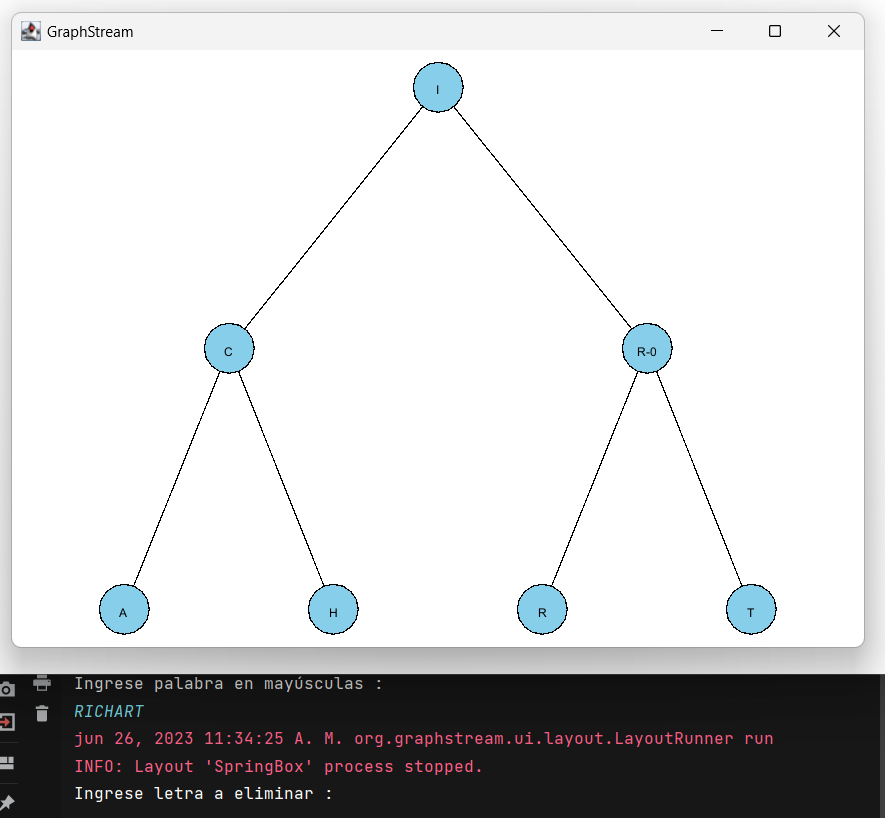
\includegraphics[width=0.7\textwidth,keepaspectratio]{img/ejecucion1.png}
	%\includesvg{img/automata.svg}
	%\label{img:mot2}
	%\caption{Product backlog.}
\end{figure}

\begin{figure}[H]
	\centering
	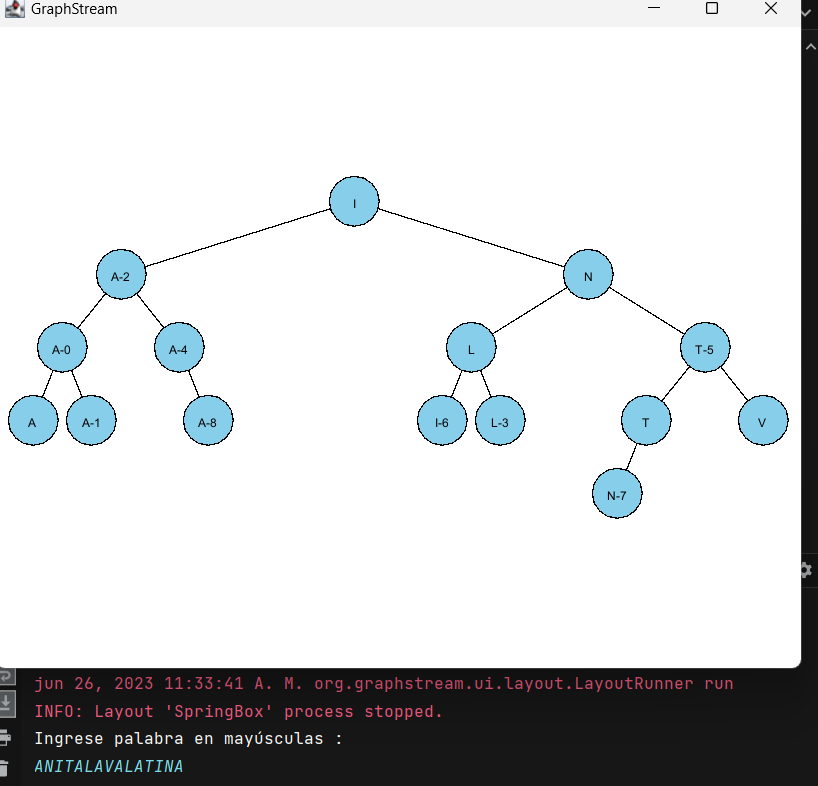
\includegraphics[width=0.7\textwidth,keepaspectratio]{img/ejecucion 2.png}
	%\includesvg{img/automata.svg}
	%\label{img:mot2}
	%\caption{Product backlog.}
\end{figure}

%%%%%%%%%%%%%%%%%%%%%%%%%%%%%%%%%%%%%%%%%%%%%%%%%%%%%%%%%%%%%%%%%%%%%%%%%%%%%%%%%%


	\subsection{Commits del trabajo}
	\begin{itemize}	
		\item Acá estan algunos de los commits mas importantes en este trabajo:
	\end{itemize}	
	
	\begin{figure}[H]
		\centering
		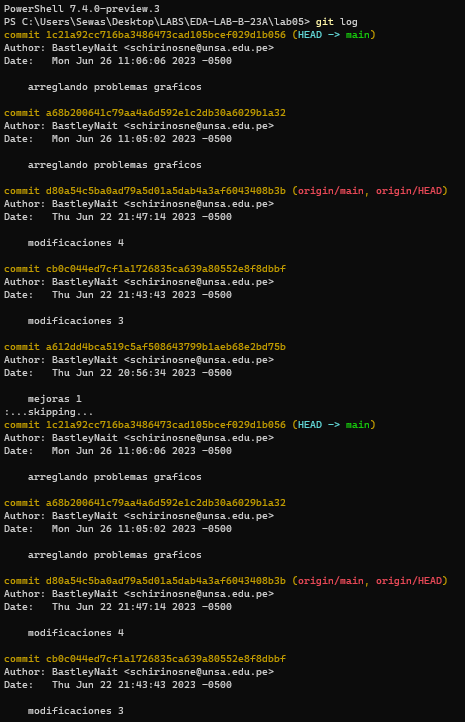
\includegraphics[width=0.7\textwidth,keepaspectratio]{img/Commits.png}
		%\includesvg{img/automata.svg}
		%\label{img:mot2}
		%\caption{Product backlog.}
	\end{figure}


%%%%%%%%%%%%%%%%%%%%%%%%%%%%%%%%%%%%%%%%%%%%%%%%%%%%%%%%%%%%%%%%%%%%%%%%%%%%%%%%%%
	
		
	\subsection{Estructura de laboratorio 05}
	\begin{itemize}	
		\item El contenido que se entrega en este laboratorio es el siguiente:
	\end{itemize}
	
\begin{lstlisting}[style=ascii-tree]
lab05/
|   .gitignore
|   AVL.java
|   Nodo.java
|   Aplicacion.java

\---latex
    |	EDA_lab05_schirinosne.pdf
    |   EDA_lab05_schirinosne.tex
    |
    +---img
    |       Commits.png
    |       ejecucion1.png
	|       ejecucion2.png
    |       logo_abet.png
    |       logo_episunsa.png
    |       logo_unsa.jpg
    |
    \---src
	|		AVL.java
	|		Nodo.java
	|		Aplicacion.java
	|		
	\---myExceptions
			ExceptionIsEmpty.java
			ExceptionNoFound.java
               
\end{lstlisting}    


	\section{\textcolor{red}{Rúbricas}}
	
	\subsection{\textcolor{red}{Entregable Informe}}
	\begin{table}[H]
		\caption{Tipo de Informe}
		\setlength{\tabcolsep}{0.5em} % for the horizontal padding
		{\renewcommand{\arraystretch}{1.5}% for the vertical padding
		
		\begin{tabular}{|p{3cm}|p{12cm}|}
			\hline
			\multicolumn{2}{|c|}{\textbf{\textcolor{red}{Informe}}}  \\
			\hline 
			\textbf{\textcolor{red}{Latex}} & \textcolor{blue}{El informe está en formato PDF desde Latex,  con un formato limpio (buena presentación) y facil de leer.}   \\ 
			\hline 
			
			
		\end{tabular}
	}
	\end{table}
	\subsection{\textcolor{red}{Rúbrica para el contenido del Informe y demostración}}
	\begin{itemize}			
		\item El alumno debe marcar o dejar en blanco en celdas de la columna \textbf{Checklist} si cumplio con el ítem correspondiente.
		\item Si un alumno supera la fecha de entrega,  su calificación será sobre la nota mínima aprobada, siempre y cuando cumpla con todos lo items.
		\item El alumno debe autocalificarse en la columna \textbf{Estudiante} de acuerdo a la siguiente tabla:
	
		\begin{table}[ht]
			\caption{Niveles de desempeño}
			\begin{center}
			\begin{tabular}{ccccc}
    			\hline
    			 & \multicolumn{4}{c}{Nivel}\\
    			\cline{1-5}
    			\textbf{Puntos} & Insatisfactorio 25\%& En Proceso 50\% & Satisfactorio 75\% & Sobresaliente 100\%\\
    			\textbf{2.0}&0.5&1.0&1.5&2.0\\
    			\textbf{4.0}&1.0&2.0&3.0&4.0\\
    		\hline
			\end{tabular}
		\end{center}
	\end{table}	
	
	\end{itemize}
	
	\begin{table}[H]
		\caption{Rúbrica para contenido del Informe y demostración}
		\setlength{\tabcolsep}{0.5em} % for the horizontal padding
		{\renewcommand{\arraystretch}{1.5}% for the vertical padding
		%\begin{center}
		\begin{tabular}{|p{2.7cm}|p{7cm}|x{1.3cm}|p{1.2cm}|p{1.5cm}|p{1.1cm}|}
			\hline
    		\multicolumn{2}{|c|}{Contenido y demostración} & Puntos & Checklist & Estudiante & Profesor\\
			\hline
			\textbf{1. GitHub} & Hay enlace URL activo del directorio para el  laboratorio hacia su repositorio GitHub con código fuente terminado y fácil de revisar. &2 &X &2 & \\ 
			\hline
			\textbf{2. Commits} &  Hay capturas de pantalla de los commits más importantes con sus explicaciones detalladas. (El profesor puede preguntar para refrendar calificación). &4 & x&4 & \\ 
			\hline 
			\textbf{3. Código fuente} &  Hay porciones de código fuente importantes con numeración y explicaciones detalladas de sus funciones. &2 &X &2 & \\ 
			\hline 
			\textbf{4. Ejecución} & Se incluyen ejecuciones/pruebas del código fuente  explicadas gradualmente. &2 &X &2 & \\ 
			\hline			
			\textbf{5. Pregunta} & Se responde con completitud a la pregunta formulada en la tarea.  (El profesor puede preguntar para refrendar calificación).  &2 &X &2 & \\ 
			\hline	
			\textbf{6. Fechas} & Las fechas de modificación del código fuente estan dentro de los plazos de fecha de entrega establecidos. &2 &X &1 & \\ 
			\hline 
			\textbf{7. Ortografía} & El documento no muestra errores ortográficos. &2 &X &2 & \\ 
			\hline 
			\textbf{8. Madurez} & El Informe muestra de manera general una evolución de la madurez del código fuente,  explicaciones puntuales pero precisas y un acabado impecable.   (El profesor puede preguntar para refrendar calificación).  &4 &x &4 & \\ 
			\hline
			\multicolumn{2}{|c|}{\textbf{Total}} &20 & &19 & \\ 
			\hline
		\end{tabular}
		%\end{center}
		%\label{tab:multicol}
		}
	\end{table}
	
\clearpage		
\section{Referencias}
\begin{itemize}			
	\item \url{https://www.geeksforgeeks.org/introduction-to-avl-tree/}
	\item \url{https://www.geeksforgeeks.org/insertion-in-an-avl-tree/}
	\item \url{https://www.geeksforgeeks.org/deletion-in-an-avl-tree/}
	\item \url{https://docs.oracle.com/javase/tutorial/java/generics/types.html}
	\item \url{https://algorithmtutor.com/Data-Structures/Tree/AVL-Trees/}

\end{itemize}	

	
%\clearpage
%\bibliographystyle{apalike}
%\bibliographystyle{IEEEtranN}
%\bibliography{bibliography}
			
\end{document}